\documentclass{article}

\usepackage{url}
\usepackage{microtype}
\usepackage{parskip}
\usepackage[super]{natbib}
\usepackage[a4paper, left=2.5cm, right=2.5cm, top=2.5cm, bottom=2.5cm]{geometry}
\usepackage{longtable,booktabs}
\usepackage{caption}
\usepackage{blindtext}
\usepackage{graphicx}
\usepackage{authblk}
\usepackage{amsmath}
\usepackage{lineno}
\usepackage[toc,page]{appendix}
\usepackage[utf8]{inputenc}
\usepackage{array} %for the tables in appendix
\usepackage{tabularx} %for the tables in appendix

%for algorithms
%\usepackage[ruled,vlined]{algorithm2e}

\usepackage{multicol}
\setlength{\columnsep}{5mm} %column separation

%working title...
\title{Introduction to QGIS (v3.14).\\
	\vspace{0.5cm}
	\large{Schedule and exercises}}
\author[1]{Kerry Pearn (k.pearn@exeter.ac.uk)}

%\affil[1]{\footnotesize University of Exeter Medical School \& NIHR South West Peninsula Applied Research Collaboration (ARC).}
%\affil[1]{\footnotesize Corresponding author: k.pearn@exeter.ac.uk}

\begin{document}
	
\maketitle
	
\section{Schedule} 
	
Today's session: 13:30 - 16:30

\emph{Format:} Today's material is fully documented in the handout "201027\_QGIS\_training\_with\_PenCHORD". I will present some QGIS functionality (for up to 20 mins) by following the material in the handout. You will then have time to work through the same part of the handout to replicate what I've just demonstrated (for up to 30 mins). You will have support on Slack from your peers and members of the PenCHORD team. %Please use us if you need help by posting any questions you have (referencing the numbered point you are working on).

\emph{Itinerary:}
\begin{itemize}
	\item \emph{Section 1 (13:30 - 13:45):} Introduction to the session and datasets 
%	\begin{itemize}
%		\item slides and data (15 mins)
%	\end{itemize}
		
	\item \emph{Section 2 (13:45 - 14:25):} The QGIS environment, map navigation \& adding your first layer 
	\begin{itemize}
		\item QGIS demo (20 mins). Exercise (20 mins)
	\end{itemize}
	
	\item \emph{Section 3 (14:25 - 14:55):} Using simple symbology
	\begin{itemize}
		\item QGIS demo (15 mins). Exercise (15 mins)
	\end{itemize}
	
	\item \emph{Break until 15:15}

	\item \emph{Section 4 (15:15 - 15:35):} Point data \& using categorized symbology
	\begin{itemize}
		\item QGIS demo (10 mins). Exercise (10 mins)
	\end{itemize}
	
	\item \emph{Section 5 (15:35 - 16:25):} Join own data to Shapefile \& using graduated symbology
	\begin{itemize}
		\item QGIS demo (20 mins). Exercise (30 mins)
	\end{itemize}
	
	\item \emph{Section 6 (16:25 - 16:30):} Print layout
	\begin{itemize}
		\item QGIS demo (5 mins).
	\end{itemize}

	\item \emph{End (16:30)}
\end{itemize}

\newpage

\section{Exercise 1.}
\textbf{Aim}: Become familiar with the relationship between the representation of the layer on the map canvas and in the attribute table.\\

Work through the notes from \emph{Chapters 2 - 5} to become familiar with the QGIS environment.

\begin{enumerate}
	\item Add the suggested toolbars
	\item Add the suggested panels
	\item Add the world basemap
	\item Practice your map navigation skills
	\item Open \& dock the attribute table for world layer
	\item Practice identifying a specific row in the attribute table with the corresponding polygon in the map canvas, and vice versa.
	\item Save project. Close QGIS. Reopen QGIS your project.
\end{enumerate}

\textbf{Result}: At the end this exercise your QGIS project should show the useful toolboxes and panels, a single layer (world) listed in the layers panel, the world layer in full zoom on the map canvas, and the world layer's attribute table docked to the bottom of the map canvas.\\


\begin{figure}[!h]
	\centering
	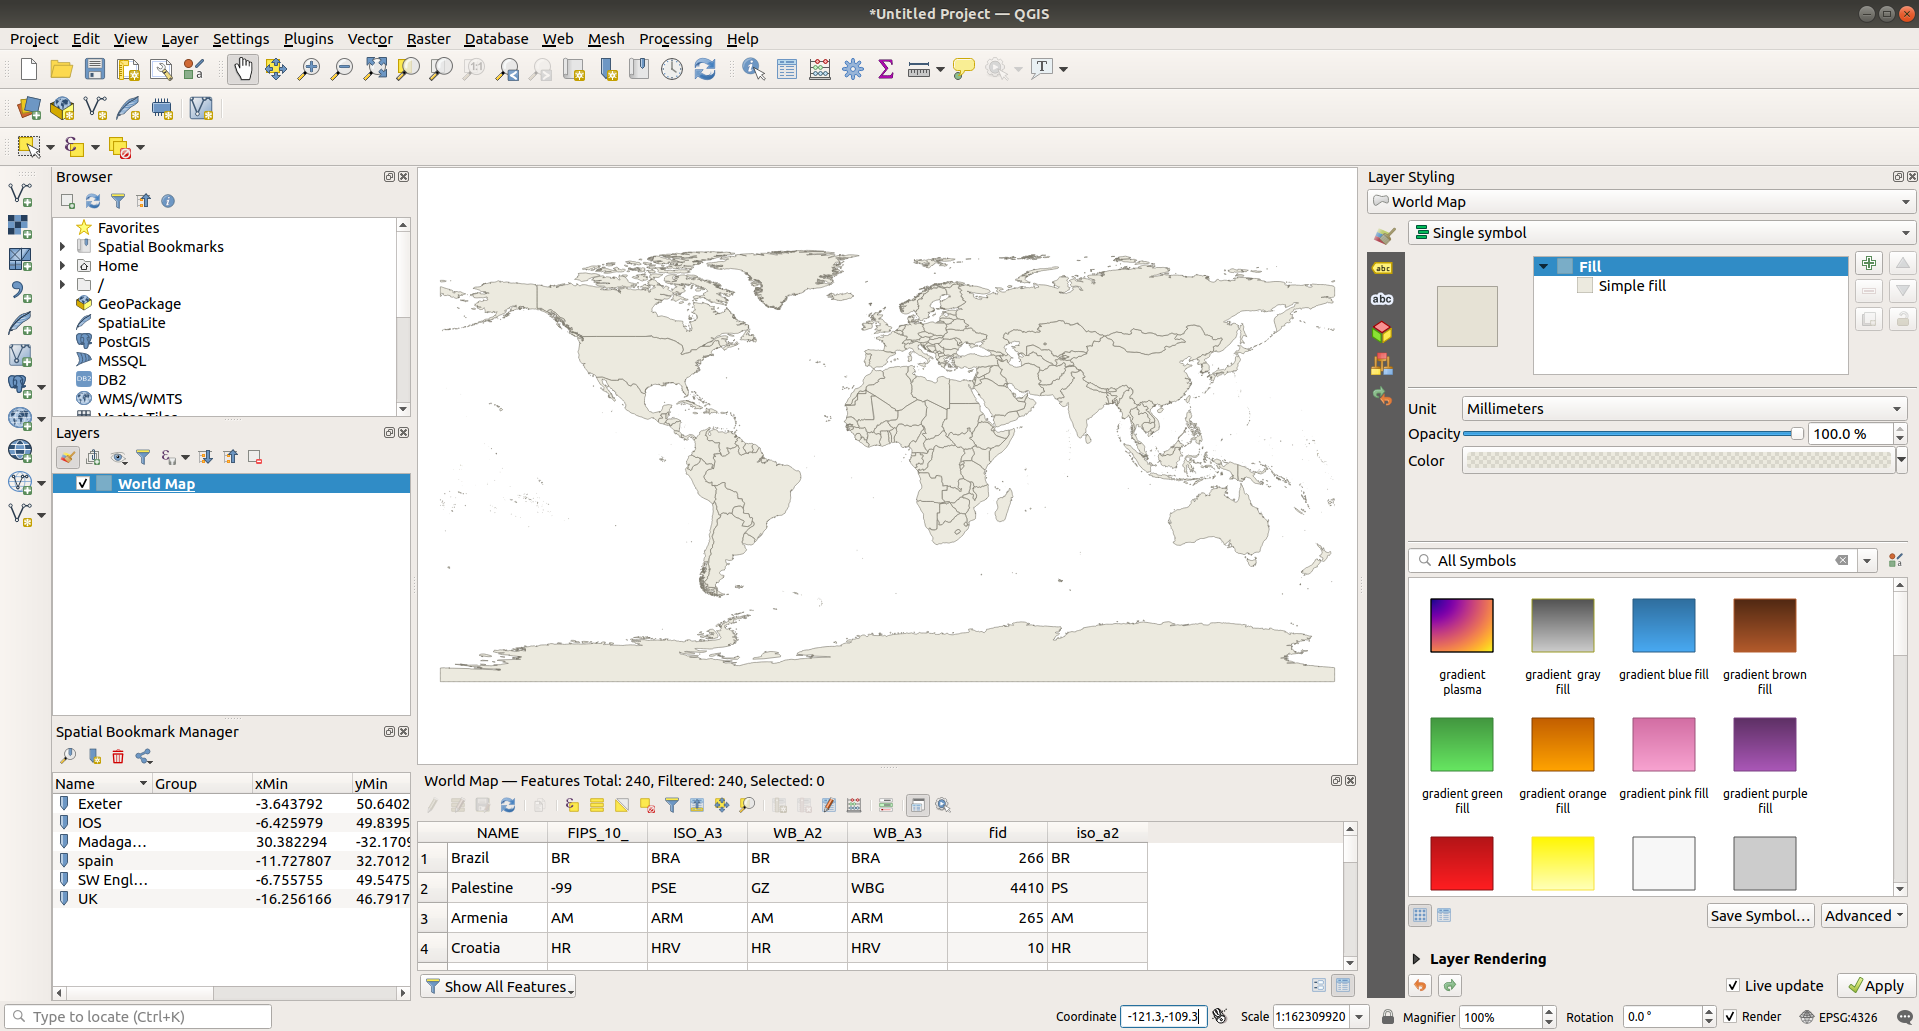
\includegraphics[width=1\textwidth]{images/exercise_1.png}
	%\caption{Rule-based styling}
	\label{ft_fig_firstfig3}
\end{figure}
\newpage

\section{Exercise 2.}
\textbf{Aim}: Extract some features from the world layer, and save them as a new shapefile. Become familiar with the \textit{Layers Styling} panel in order to change the appearance of the layer using simple symbology.\\

Work through the notes from \emph{Chapter 6 - 8} to save a new shapefile (just the UK) and add simple styling. The steps that you will cover are:

\begin{enumerate}
	\item Change the project projection to EPSG: 32630 (see chapter 6).
	\item From the world layer, select polygons for UK. These are now your "selected features" (see chapter 7).
	\item Export selected features to new shapefile called "UK.shp" (see chapter 7).
	\item Play with the order of the two layers in the layers panel (world and UK). Toggle between having both/one/none selected (please end with the UK being the only one selected, and zoom to this layer)
	\item Customise the simple symbology for the UK shapefile (follow Chapter 8). 
\end{enumerate}

\textbf{Result}: At the end this exercise your QGIS project should show the UK as land and coast.\\


\begin{figure}[!h]
	\centering
	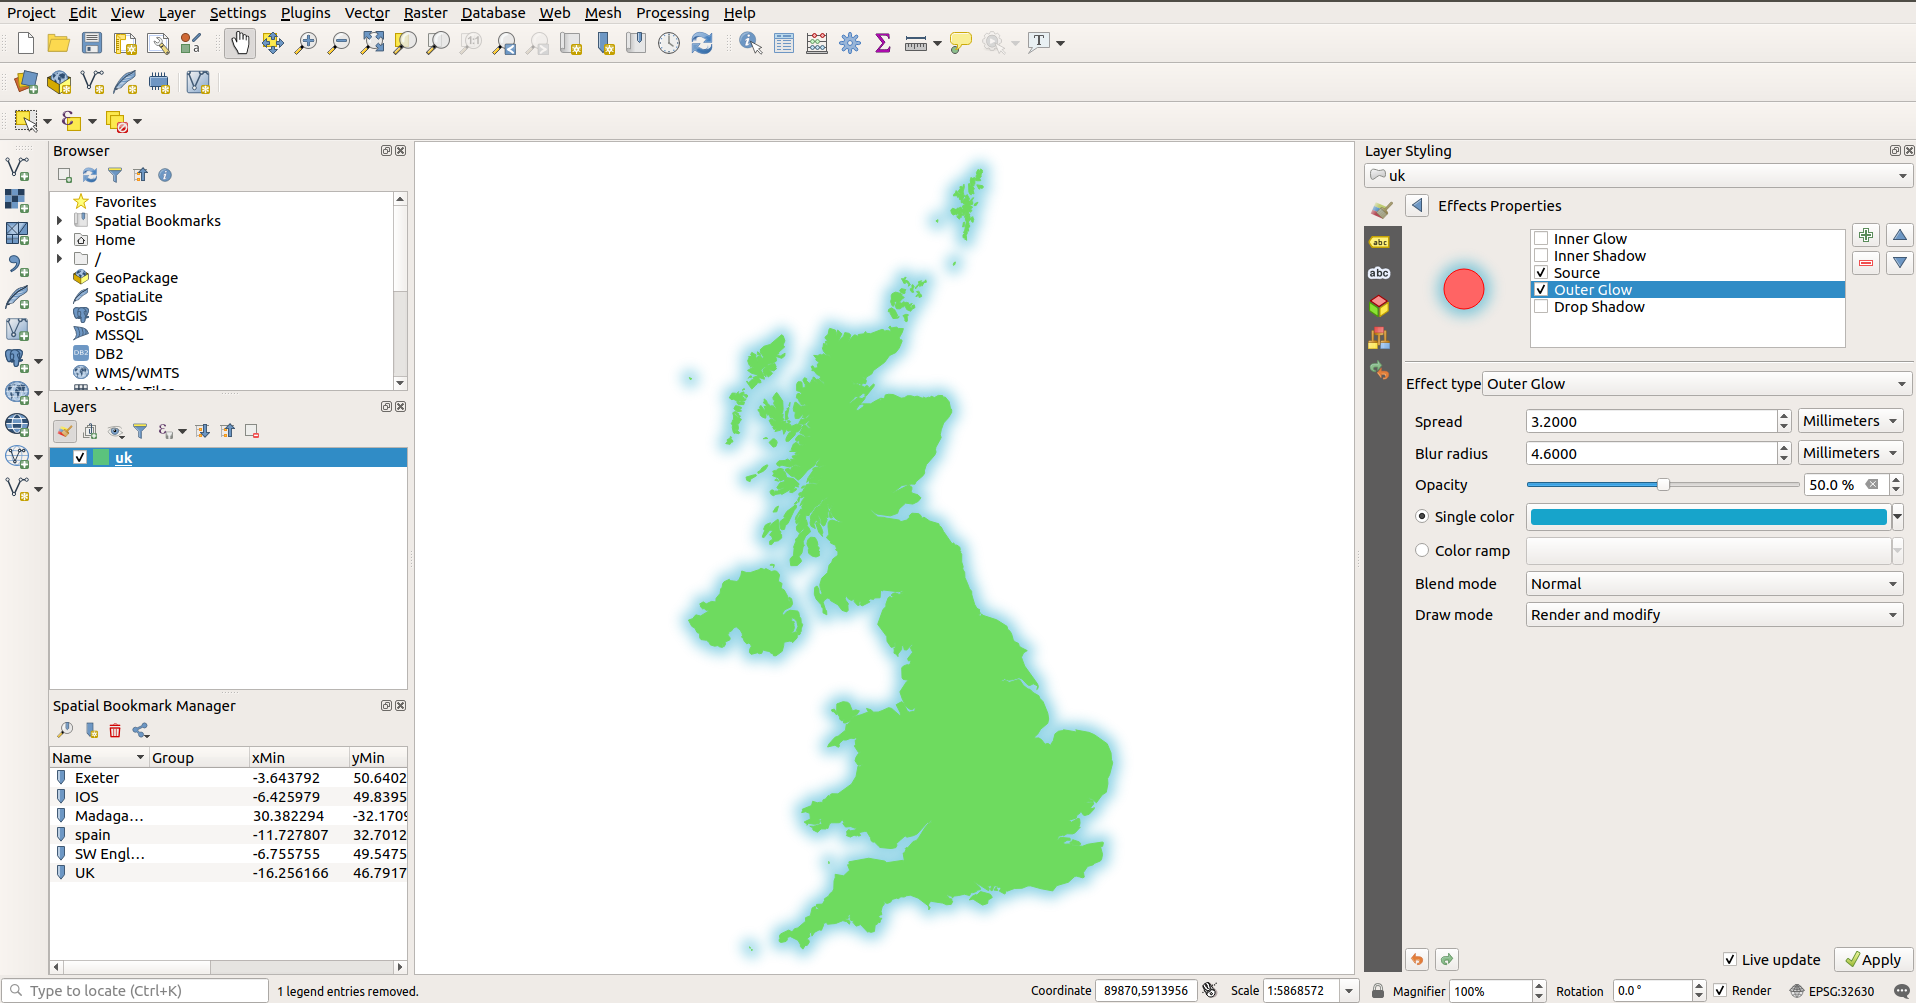
\includegraphics[width=1\textwidth]{images/exercise_2.png}
	\caption{Exercise 2}
	\label{ft_fig_firstfig3}
\end{figure}

\newpage
\section{Exercise 3}

\textbf{Aim}: Add point data from a delimited text file (.csv) and style the points using categorised symbology\\
 
\textbf{Exercise 3A}: Follow \emph{Chapter 11.}. Add your Police HQ point data and style each point to represent whether the site is also a Fire and Rescue HQ. 

\textbf{Exercise 3B}: Follow \emph{Chapter 12.}. Add a label to each point to state the site's location (using field "Head quarters").

\textbf{Result}: At the end this exercise your QGIS project should show the UK basemap, with 5 points for the locations of the Police headquarters, points styled based on site type, and a label showing the site name.\\


\begin{figure}[!h]
	\centering
	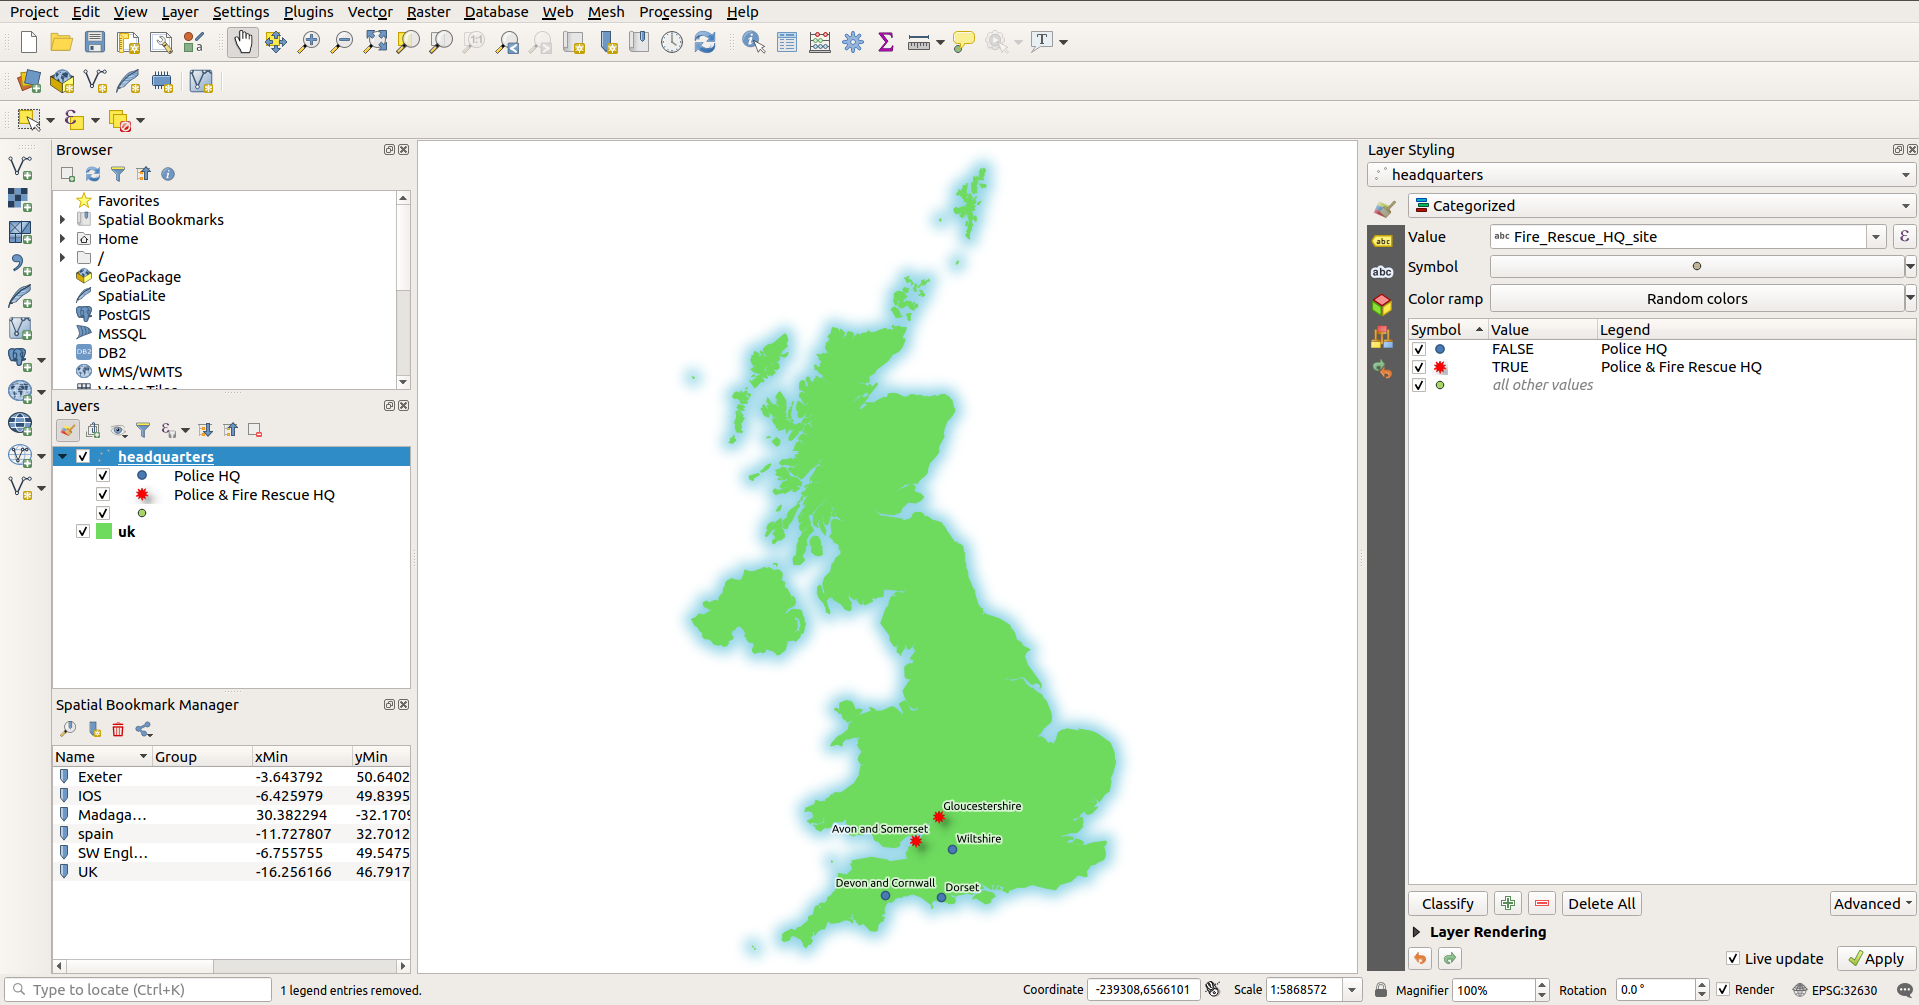
\includegraphics[width=1\textwidth]{images/exercise_3.png}
	\caption{Exercise 3}
	\label{ft_fig_firstfig3}
\end{figure}

\newpage
\section{Exercise 4}

\textbf{Aim}: Become familiar with joining your own data (.csv file) to a corresponding shapefile in order to visualise your data. Use continuous symbology to style the layer.\\

\textbf{Exercise 4A:} Follow notes from \emph{Chapter 13 \& 14} to i) add delimited text file ii) add shapefile and 3) create a table join.

\textbf{Exercise 4B:} Using the information covered in \emph{Chapter 15}, choose two columns from the street crime dataset and style them using graduated symbology. Duplicate the layer so that a separate layer is displaying each column (rename each layer).

\textbf{Result}: At the end this exercise your QGIS project should show LSOA crime data for the SW, styled to represent a data field, together with a UK basemap \& the 5 locations of the Police headquarters. 
\\


\begin{figure}[!h]
	\centering
	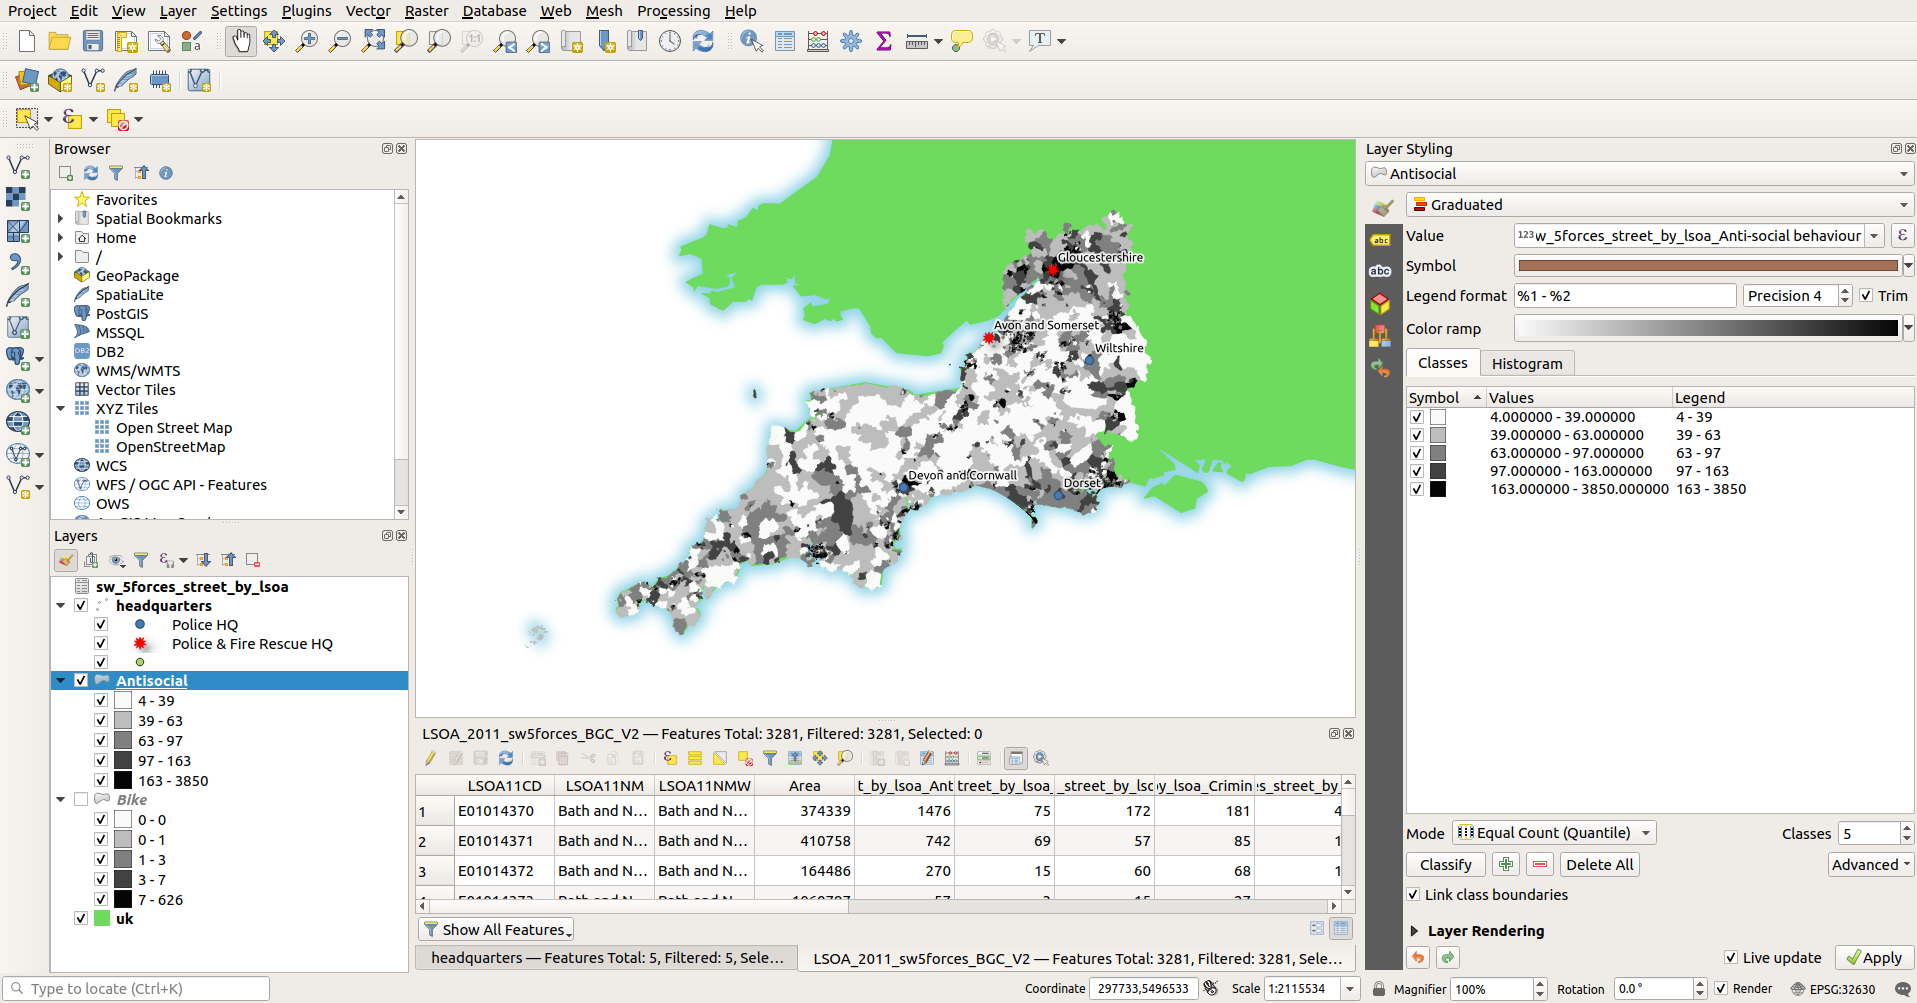
\includegraphics[width=1\textwidth]{images/exercise_4.png}
	\caption{Exercise 4}
	\label{ft_fig_firstfig3}
\end{figure}

\end{document}
